% Options for packages loaded elsewhere
\PassOptionsToPackage{unicode}{hyperref}
\PassOptionsToPackage{hyphens}{url}
\documentclass[
  ignorenonframetext,
  twocolumn]{beamer}
\newif\ifbibliography
\usepackage{pgfpages}
\setbeamertemplate{caption}[numbered]
\setbeamertemplate{caption label separator}{: }
\setbeamercolor{caption name}{fg=normal text.fg}
\beamertemplatenavigationsymbolsempty
% remove section numbering
\setbeamertemplate{part page}{
  \centering
  \begin{beamercolorbox}[sep=16pt,center]{part title}
    \usebeamerfont{part title}\insertpart\par
  \end{beamercolorbox}
}
\setbeamertemplate{section page}{
  \centering
  \begin{beamercolorbox}[sep=12pt,center]{section title}
    \usebeamerfont{section title}\insertsection\par
  \end{beamercolorbox}
}
\setbeamertemplate{subsection page}{
  \centering
  \begin{beamercolorbox}[sep=8pt,center]{subsection title}
    \usebeamerfont{subsection title}\insertsubsection\par
  \end{beamercolorbox}
}
% Prevent slide breaks in the middle of a paragraph
\widowpenalties 1 10000
\raggedbottom
\AtBeginPart{
  \frame{\partpage}
}
\AtBeginSection{
  \ifbibliography
  \else
    \frame{\sectionpage}
  \fi
}
\AtBeginSubsection{
  \frame{\subsectionpage}
}
\usepackage{iftex}
\ifPDFTeX
  \usepackage[T1]{fontenc}
  \usepackage[utf8]{inputenc}
  \usepackage{textcomp} % provide euro and other symbols
\else % if luatex or xetex
  \usepackage{unicode-math} % this also loads fontspec
  \defaultfontfeatures{Scale=MatchLowercase}
  \defaultfontfeatures[\rmfamily]{Ligatures=TeX,Scale=1}
\fi
\usepackage{lmodern}
\usetheme[]{tud}
\ifPDFTeX\else
  % xetex/luatex font selection
\fi
% Use upquote if available, for straight quotes in verbatim environments
\IfFileExists{upquote.sty}{\usepackage{upquote}}{}
\IfFileExists{microtype.sty}{% use microtype if available
  \usepackage[]{microtype}
  \UseMicrotypeSet[protrusion]{basicmath} % disable protrusion for tt fonts
}{}
\makeatletter
\@ifundefined{KOMAClassName}{% if non-KOMA class
  \IfFileExists{parskip.sty}{%
    \usepackage{parskip}
  }{% else
    \setlength{\parindent}{0pt}
    \setlength{\parskip}{6pt plus 2pt minus 1pt}}
}{% if KOMA class
  \KOMAoptions{parskip=half}}
\makeatother
% definitions for citeproc citations
\NewDocumentCommand\citeproctext{}{}
\NewDocumentCommand\citeproc{mm}{%
  \begingroup\def\citeproctext{#2}\cite{#1}\endgroup}
\makeatletter
 % allow citations to break across lines
 \let\@cite@ofmt\@firstofone
 % avoid brackets around text for \cite:
 \def\@biblabel#1{}
 \def\@cite#1#2{{#1\if@tempswa , #2\fi}}
\makeatother
\newlength{\cslhangindent}
\setlength{\cslhangindent}{1.5em}
\newlength{\csllabelwidth}
\setlength{\csllabelwidth}{3em}
\newenvironment{CSLReferences}[2] % #1 hanging-indent, #2 entry-spacing
 {\begin{list}{}{%
  \setlength{\itemindent}{0pt}
  \setlength{\leftmargin}{0pt}
  \setlength{\parsep}{0pt}
  % turn on hanging indent if param 1 is 1
  \ifodd #1
   \setlength{\leftmargin}{\cslhangindent}
   \setlength{\itemindent}{-1\cslhangindent}
  \fi
  % set entry spacing
  \setlength{\itemsep}{#2\baselineskip}}}
 {\end{list}}
\usepackage{calc}
\newcommand{\CSLBlock}[1]{\hfill\break\parbox[t]{\linewidth}{\strut\ignorespaces#1\strut}}
\newcommand{\CSLLeftMargin}[1]{\parbox[t]{\csllabelwidth}{\strut#1\strut}}
\newcommand{\CSLRightInline}[1]{\parbox[t]{\linewidth - \csllabelwidth}{\strut#1\strut}}
\newcommand{\CSLIndent}[1]{\hspace{\cslhangindent}#1}
\setlength{\emergencystretch}{3em} % prevent overfull lines
\providecommand{\tightlist}{%
  \setlength{\itemsep}{0pt}\setlength{\parskip}{0pt}}
% Use fontspec to load Noto Emoji
\usepackage{fontspec}

% Define Noto Emoji font for emojis
\newfontfamily\emojiFont{Noto Emoji}
\newfontfamily\fallbackFont{DejaVu Sans}

% Automatically switch to emoji font for unicode emoji characters
\newcommand{\emoji}[1]{{\emojiFont #1}}
% Command for fallback font
\newcommand{\fallback}[1]{{\fallbackFont #1}}

\usepackage{bookmark}
\IfFileExists{xurl.sty}{\usepackage{xurl}}{} % add URL line breaks if available
\urlstyle{same}
\hypersetup{
  pdftitle={Is 5G a Battery Drainer?},
  pdfauthor={Alexander Kusnezoff},
  hidelinks,
  pdfcreator={LaTeX via pandoc}}

\title{Is 5G a Battery Drainer?}
\author{Alexander Kusnezoff}
\date{16.07.2024}

% >>> added to default template

\title{Is 5G a Battery Drainer?}
\subtitle{}
\author{Alexander Kusnezoff}
\date{16.07.2024}

\AtBeginSection[]{
  \partpage{\usebeamertemplate***{part page}}
}
% <<< added to default template


\begin{document}

\maketitle

% 
% \frame{\titlepage}

\section{title}\label{title}

\begin{frame}{Start with Why?}
\protect\phantomsection\label{start-with-why}
Test1

\pause 

Text2
\end{frame}

\begin{frame}{Start with Why?}
\protect\phantomsection\label{start-with-why-1}
\begin{center}
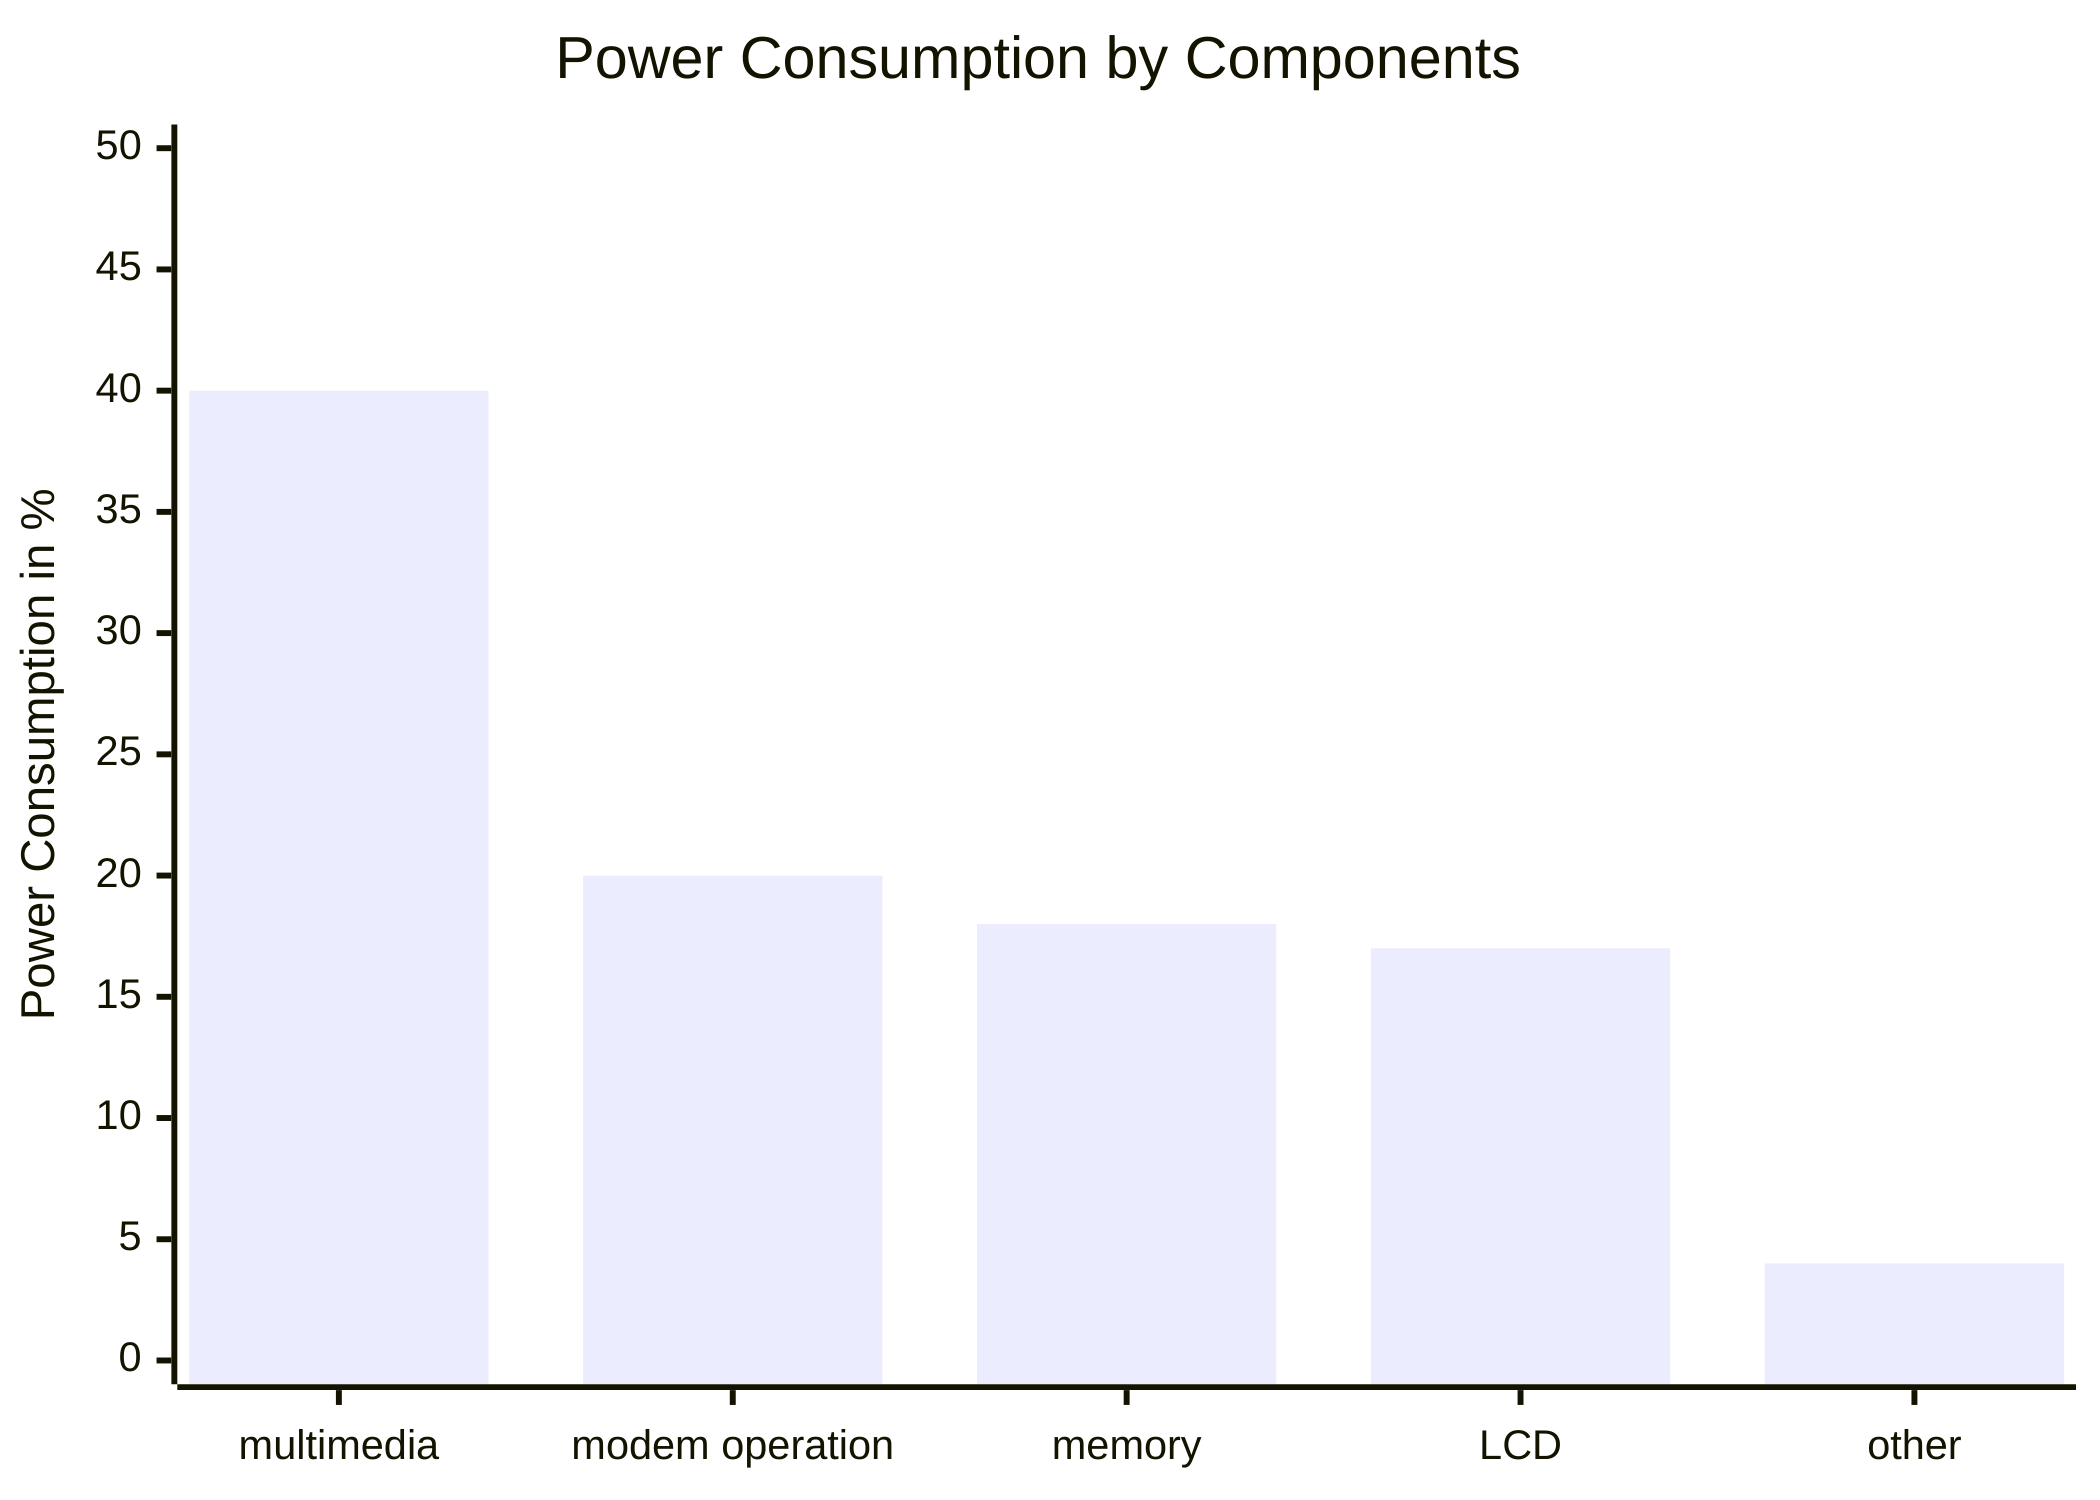
\includegraphics[width=0.8\textwidth]{./img/prosem-einleitung.png}
\end{center}
\end{frame}

\begin{frame}{Slide 3}
\protect\phantomsection\label{slide-3}
Test3
\end{frame}

\section{Neue Section}\label{neue-section}

\begin{frame}{HMMM}
\protect\phantomsection\label{hmmm}
\end{frame}

\begin{frame}{Twocols}
\protect\phantomsection\label{twocols}
This is how to specify several cols on a slide:

\begin{columns}[T]
\begin{column}{0.4\linewidth}
contents\ldots{}
\end{column}

\begin{column}{0.6\linewidth}
contents\ldots{}
\end{column}
\end{columns}
\end{frame}

\begin{frame}{References}
\protect\phantomsection\label{references}
``my quote'' \citeproc{ref-PXJVWCSQ}{{[}1{]}}
\end{frame}

\begin{frame}{Extra Symbols}
\protect\phantomsection\label{extra-symbols}
\begin{itemize}
\tightlist
\item
  \fallback{✓} \emoji{🧠}, \emoji{📙}
\end{itemize}
\end{frame}

\section{End}\label{end}

\begin{frame}{End}
\protect\phantomsection\label{refs}
\begin{CSLReferences}{0}{0}
\bibitem[\citeproctext]{ref-PXJVWCSQ}
\CSLLeftMargin{{[}1{]} }%
\CSLRightInline{F. Gao, G. Tziantzioulis, and D. Wentzlaff,
{``ComputeDRAM: In-memory compute using off-the-shelf DRAMs,''} in
\emph{Proceedings of the 52nd annual IEEE/ACM international symposium on
microarchitecture}, in MICRO '52. New York, NY, USA: Association for
Computing Machinery, Oct. 2019, pp. 100--113. doi:
\href{https://doi.org/10.1145/3352460.3358260}{10.1145/3352460.3358260}.
Available: \url{https://dl.acm.org/doi/10.1145/3352460.3358260}.
{[}Accessed: Jul. 16, 2025{]}}

\end{CSLReferences}
\end{frame}

\end{document}
